\chapter{Atmospheric Temperatures Variations}\label{ch:atm_variations}

The present chapter is devoted to the presentation of the numerical methods
and tools that has been adopted to calculate estimates of atmospsheric
brighness temperatures at our observation site. The CMB Atmospheric
Library, the software library that has been employed to perform
montecarlo simulations of the meteorological parameters and to solve the
radiative transfer equation, is introduced first. Then, our numerical
results, the seasonal matrices for atmospheric brightness
temperatures, are presented and discussed.

\section{The CMB Atmospheric Library}

The \emph{CMB Atmospheric Library}
(CAL)\footnote{\url{https://github.com/cmbgroundbased/cal}} is a free and
open source software library that has been developed to produce computer
simulations of atmospheric effects and telescope observations for
ground-based CMB experiments. CAL incorporates code extracted from the
well-known \emph{Time Ordered Astrophysics Scalable Tools} (TOAST) software
framework, making it and independent module, which can be exploited by
different CMB ground-based experiments. The CMB Atmospheric Library core is
written in \texttt{C++} programming language, in order to maintain high
performance.  However, \texttt{Python} programming language bindings are
provided to simplify its integration in experiments making use of
\texttt{Python} based pipelines.

CAL can be used to solve the atmospheric radiative transfer equation, which
has been discussed in \autoref{ss:radiative_transfer_eq}. To this end, the
library ships with
\emph{libaatm}\footnote{\url{https://github.com/hpc4cmb/libaatm}}, a
repackaged version of the \emph{Alma Atmospheric Transmission at Microwaves
Tools} (cit pardo), a model of the longwave atmospheric spectrum based on
broadband measurements and calculations. The model is fully applicable from
\SIrange{0}{2}{\tera\hertz} while including lines up to
\SI{10}{\tera\hertz}. Its primary goal is to simulate the
millimeter and submillimeter regions accessible from the ground.
libaatm discretize the atmosphere in a finite number of vertical
layers, from sea level to the tropopause, by a predefined internal profile.
Then, the radiative transfer equation is solved for each layer and
solutions are connected.

\subsection{CAL Relevant Methods}

The relevant methods which are provided by CAL and have been used in this
work follow:

\begin{itemize}
        \item \texttt{Weather}:

        This class can be initialized with the CDFs \texttt{.fits} file, which
        has been described in \autoref{s:CDF_fits_file}. It takes in input
        an UTC time structure with time resolution of \num{1} hour and
        returns pseudo-random realizations of meteorological parameters,
        determined by the probability distributions derived from the input
        \texttt{.fits} file.

        \item \texttt{atm\_atmospheric\_loading}:

        A wrapper function around libaatm methods. It solves the radiative
        transfer equation for a realization of the atmosphere defined by
        the values of $T_s$,
        $P_s$ and PWV, which are expected as input. It returns the value of sky
        brightness temperature in \si{\kelvin} (Rayleigh-Jeans) at a given
        frequency value, specified in input.

        \item \texttt{atm\_absorption\_coefficient}:

        As the latter one, this function solves the radiative transfer equation,
        but the total absorption coefficient,

        \begin{equation}
                \alpha_A\qty(\nu) = 1 - e^{-\tau_A\qty(\nu)}
        \end{equation}

        for the specified atmosphere realization at a given frequency is
        returned.
\end{itemize}

These three objects hides a significant implementation complexity, but are
simple in use. They can be jointly used to produce montecarlo simulations of
atmospheric brightness temperature at Pico del Teide, or at any other site
of interest.

%\section{The \texttt{tatmget} Computer Program}

\section{Atmospheric Temperatures Seasonal Matrices}

Atmospheric brightness temperatures can be computed starting from the
methods provided by the CMB Atmospheric Library, by making use of
\autoref{eq:rte_solution_thermal}:

\begin{equation}
        T\qty(1 - e^{-\tau_{A,\nu}})= T_b - T_b\qty(0) e^{-\tau_{A,\nu}}.
\end{equation}

The terms in the equation have been rearranged, because right now we are
not interested in the total sky brightness temperature, $T_b \equiv
T_\text{sky}$, but only in the contribution due to the atmosphere, $T\qty(1
- e^{-\tau_{A,\nu}}) \equiv T_\text{atm}$, which depends on atmospheric
physical properties. $T_b(0)$ is the brightness temperature of the incoming
cosmic radiations. If it is assumed that the instrument is observing a
relatively clear patch of sky this contribution is dominated by the cosmic
microwave background radiation. Therefore, we have:

\begin{equation}
        T_\text{atm}\qty(\nu) = T_\text{sky}\qty(\nu) -
        T_\text{CMB}\qty(\nu)e^{-\tau_A\qty(\nu)}
        \label{eq:tatm_formula}
\end{equation}

where $T_\text{CMB}\qty(\nu)$ is the CMB brightness temperature expressed
in \si{\kelvin} Rayleigh-Jeans and $\tau_A\qty(\nu)$ is the total optical
depth of the atmosphere. $T_\text{CMB}\qty(\nu)$ is diminished by an
exponential factor that depends on the total opacity.

$T_\text{sky}\qty(\nu)$ and $\tau_A\qty(\nu)$ can be computed for arbitrary
frequencies and atmosphere realizations by means of the three CAL methods
listed above. The value of $T_\text{CMB}$ has been measured with great
precision and can be easily converted in \si{\kelvin} Rayleigh-Jeans for any
given frequency.

A population of \num{1000} values of $T_\text{atm}$ at \SI{43}{\giga\hertz}
(Strip Q-band central frequency) has been computed for every hour of each
typical day of every month of the year, for a total of \num{288}
statistical populations. The \texttt{Weather} class has been initialized
with the CDFs \texttt{.fits} file, which in turn was obtained starting from
the ERA5 meteorological data for Pico del Teide. Then, each statistical
population has been subdivided into \num{10} samples of \num{100} elements
each. Expectation values for each population has been computed, using mean
and median as estimators. The corresponding standard errors have been
obtained by calculation of standard deviation of the mean, in the case of
the first estimator, and making use of a bootstrapping technique, from the
samples, in the case of the second one.

Our results are showed in \autoref{fig:tatm_nocal} and
\autoref{fig:tatm_matrices_nocal}. Median daily variations in atmospheric
brightness temperature for each month of the year are showed in
\autoref{fig:tatm_nocal}. The corresponding seasonal matrices, showing mean
and median seasonal variations in $T_\text{atm}$, are represented in
\autoref{fig:tatm_nocal}.

The annual average brightness temperature daily excursion is \SI{0.69 \pm
0.06}{\kelvin}, a small value if compared to the average annual
excursion: \SI{3.67 \pm 0.08}{\kelvin}. In particular
September, October and November are charactherized by larger values of
atmospheric brightness temperature, suggesting that bad weather days are more
frequent during these months, making them less suitable for observations.

\begin{figure}
        \centering
        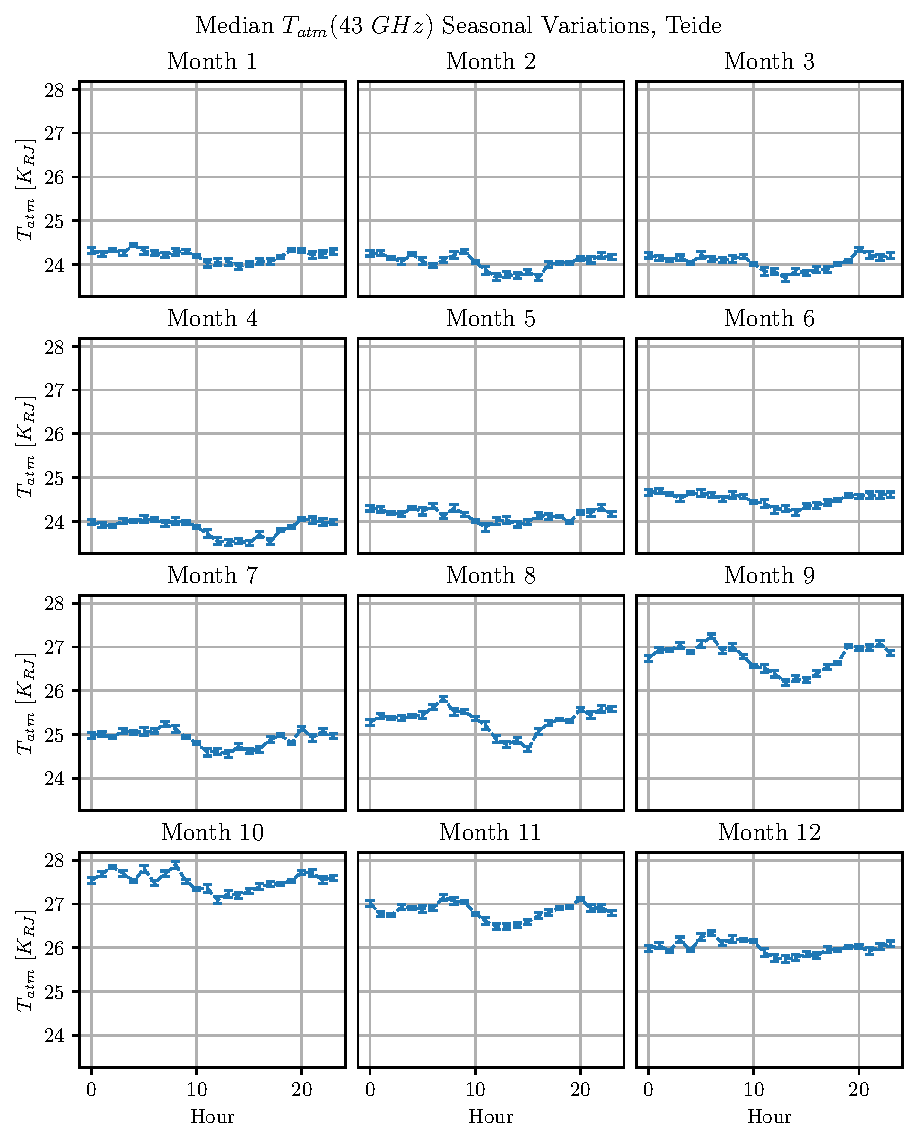
\includegraphics[width=\textwidth]{TATM_nocal}
        \caption{Median atmospheric brightness temperature seasonal variations for
        Teide}
        \label{fig:tatm_nocal}
\end{figure}

\begin{figure}
        \centering
        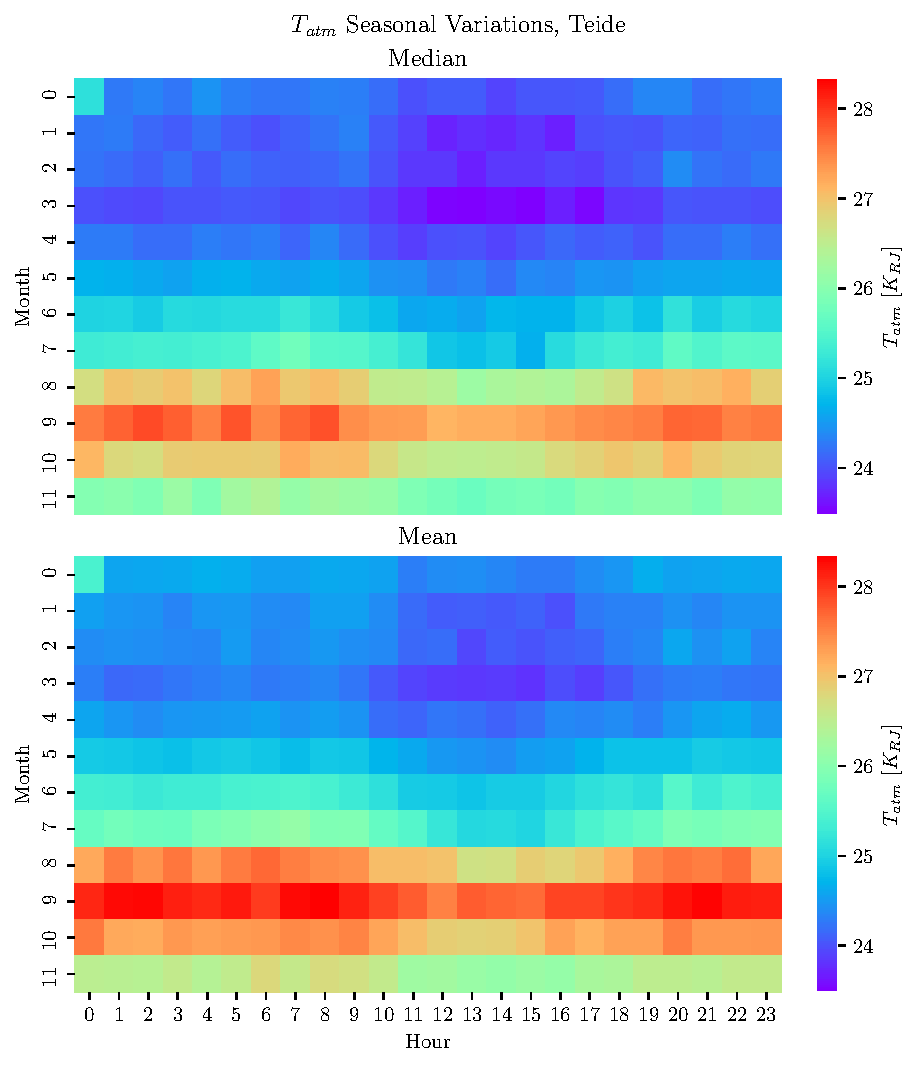
\includegraphics[width=\textwidth]{TATM_Matrices_nocal}
        \caption{$T_\text{atm}$ seasonal matrices for Teide.}
        \label{fig:tatm_matrices_nocal}
\end{figure}

